\section{Introduction}

Program verification with interactive theorem provers has come a long way since its inception,
especially when it comes to the scale of programs that can be verified.
The seL4~\cite{Klein2009} verified operating system kernel, for example,
is the effort of a team of proof engineers spanning more than
a million lines of proof, costing over 20 person-years.
Given a famous 1977 critique of verification~\cite{DeMillo1977} (emphasis ours):

\begin{quote}
A \textit{sufficiently fanatical researcher}
might be willing to devote \textit{two or 
three years} to verifying a significant 
piece of software if he could be 
assured that the software would remain stable.
\end{quote}
we could argue that, over 40 years, either verification has become easier,
or researchers have become more fanatical. Unfortunately, not all has changed (emphasis still ours):

\begin{quote}
But real-life programs need to 
be maintained and modified. 
There is \textit{no reason to believe} that verifying a modified program is any 
easier than verifying the original the 
first time around.
\end{quote}
Tools that can automatically refactor or repair proofs~\cite{wibergh2019, WhitesidePhD, Dietrich2013, adams2015, Bourke12, Roe2016, robert2018, pumpkinpatch}
give us reason to believe that verifying a modified program \textit{can} sometimes be easier than verifying the original, even when proof engineers do not follow good development processes,
or when change occurs outside of proof engineers' control~\cite{PGL-045}.
Still, maintaining verified programs can be challenging: it means keeping not just the programs, but also specifications and proofs about those programs up-to-date.
This remains so difficult that sometimes, even experts give up in the face of change~\cite{replica}.

The problem of automatically updating proofs in response to changes in programs or specifications is known as \textit{proof repair}~\cite{PGL-045, pumpkinpatch}.
While there are many ways proofs need to be repaired, one is in response to a changed type definition (Section~\ref{sec:key1}).
We make progress on two open challenges in proof repair in response to changes in type definitions:

\begin{enumerate}
\item Existing work supports very limited classes of these changes like non-structural changes~\cite{pumpkinpatch} or a predefined set
of changes~\cite{robert2018, wibergh2019}, and these are not informed by the needs of proof engineers~\cite{replica}.
\item Proof repair tools are not yet integrated with typical proof engineering workflows like tactics~\cite{PGL-045, pumpkinpatch, robert2018},
and may impose additional proof obligations like proving relations corresponding to changes~\cite{Ringer2019}.
\end{enumerate}
%Our progress towards these challenges leverages three key insights:%
%
%\begin{enumerate}
%\item Proof repair is a form of proof reuse---reusing proofs about one specification to derive proofs about another specification---with 
%the additional challenge that one of the specifications may cease to exist.
%The key to supporting proof repair is to build a proof reuse
%tool that can handle that additional challenge (Section~\ref{sec:key1}). 
%\item A configurable proof term transformation can be used to build such a proof repair tool,
%and the result can handle many different kinds of changes (Section~\ref{sec:key2}).
%\item The transformed proof terms can then be translated back to suggested tactic scripts (Section~\ref{sec:decompiler}).
%\end{enumerate}

Our approach combines a configurable proof term transformation (Section~\ref{sec:key2}) with a prototype decompiler from proof terms
back to suggested tactics (Section~\ref{sec:decompiler}). % TODO mention search or not?
This is implemented (Section~\ref{sec:impl}) in \toolname\footnote{Name changed for double-blind.} (Configurable Approach to Repairing \& Refactoring Outdated Tactics), a proof repair plugin for Coq 8.8 that is available on Github.\footnote{For double-blind, we annotate each claim to which code is relevant with a circled number like \circled{1}. \lstinline{GUIDE.md} in auxiliary material maps these to code.}
%The result is a flexible proof repair tool that: 

%\begin{enumerate}
%\item supports changes in types informed by proof engineers and not supported by other tools, and
%\item suggests tactic scripts and proves relations corresponding to certain changes for better workflow integration.
%\end{enumerate}

\mysubsubsec{Addressing Challenge 1: Flexible Type Support}
The case studies in Section~\ref{sec:search}---summarized in Table~\ref{fig:changes}---show that \toolname is flexible enough to support
a wide range of proof engineering use cases. % can support a flexible class of changes informed by the needs of proof engineers within a unified framework.
In general, \toolname can support any change described by an equivalence, though it takes the equivalence in a
deconstructed form that we call a \textit{configuration}.
The configuration expresses to the proof term transformation how to translate functions and proofs defined over the old version of a type
to refer only to the new version, and how to do so in a way that does not break definitional equality.
The proof engineer can write this configuration in Coq and feed it to \toolname (\textit{manual configuration} in Table~\ref{fig:changes}),
configuring \toolname to support the corresponding change. %from directly within Coq.

\mysubsubsec{Addressing Challenge 2: Workflow Integration}
Research on workflow integration for proof repair tools is in its infancy.
\toolname is built with workflow integration in mind.
For example, \toolname is the only proof repair tool we are aware of that produces suggested tactic scripts for repaired proofs,
a challenge highlighted in existing proof repair work~\cite{pumpkinpatch, robert2018} and in 
a recent survey of proof engineering~\cite{PGL-045}.
In addition, \toolname implements search procedures that 
automatically discover configurations and prove the equivalences they induce for four different classes of 
changes (\textit{automatic configuration} in Table~\ref{fig:changes}),
decreasing the burden of proof obligations imposed on the proof engineer.
Our partnership with an industrial proof engineer\footnote{Note for double-blind: the anonymized proof engineer is not an author.} has informed other changes to further improve workflow integration
(Sections~\ref{sec:implementation} and~\ref{sec:search}).

\begin{figure}
%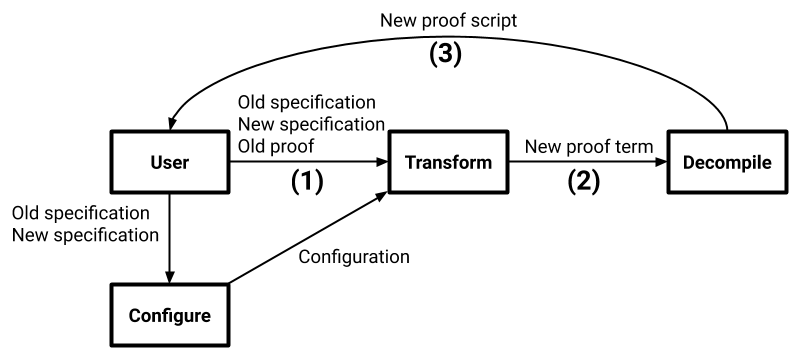
\includegraphics[width=\columnwidth]{workflowa.pdf}
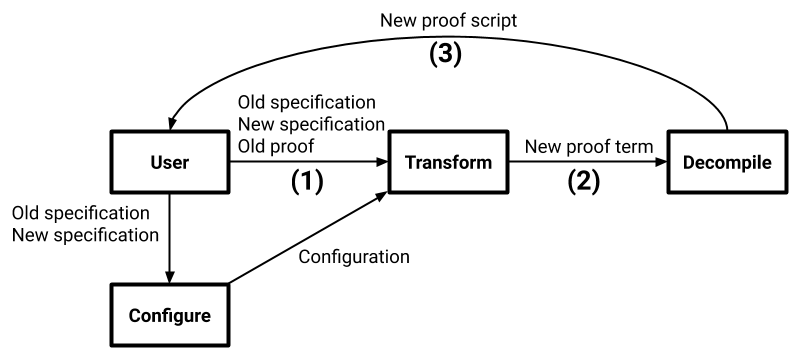
\includegraphics[width=\columnwidth]{workflowa.pdf}
\vspace{-0.7cm}
\caption{The workflow for \toolname.}
\vspace{-0.1cm}
\label{fig:system}
\end{figure}

\mysubsubsec{Bringing it Together}
Figure~\ref{fig:system} shows how this comes together when the proof engineer invokes \toolname:

\begin{enumerate}
\item The proof engineer \textbf{Configure}s \toolname, either manually or automatically.
\item The configured \textbf{Transform} transforms the old proof term into the new proof term.
\item \textbf{Decompile} suggests a new proof script. % given the new proof term.
\end{enumerate}
There are currently four search procedures for automatic configuration implemented in \toolname (see Table~\ref{fig:changes}).
%All four search procedures generate equivalence proofs as in Figure~\ref{fig:equivalence} automatically (\href{https://github.com/uwplse/pumpkin-pi/%blob/master/plugin/src/automation/search/search.ml}{search.ml} and \href{https://github.com/uwplse/pumpkin-pi/blob/master/plugin/src/automation/search/equivalence.ml}{equivalence.ml}),
%then configure (\href{https://github.com/uwplse/pumpkin-pi/blob/master/plugin/src/automation/lift/liftconfig.ml}{liftconfig.ml}) the transformation %to those equivalences.
Manual configuration makes it possible
for the proof engineer to configure the transformation to any other equivalence,
even without a search procedure.
Section~\ref{sec:search} shows examples of both workflows applied to real scenarios.

%Our main technical advances are techniques for transforming proof terms directly to repair broken proofs in response to changes
%in types, while our prototype decompiler up to tactics is important for usability in Coq.
%We elaborate on some of the examples from Table~\ref{fig:changes} to further demonstrate flexibility and usability with four case studies (Section~%\ref{sec:search}), which show that \toolname 1) can support a benchmark from a user study of Coq proof engineers, 2) can simplify dependently-typed programming, %automating manual steps from previous work,
%3) can help proof engineers port functions and proofs from unary to binary numbers, and
%4) has helped an industrial proof engineer at Galois integrate Coq with a company workflow and write proofs about an implementation of the TLS %Handshake Protocol.

